\chapter[Design of a Flexible Visual Debugging System]{Design of a Flexible Visual\\Debugging System}
\label{visual_debugging_system}

Debugging in robotics has unique requirements which are often not met by traditional debugging systems. The special requirements lead to a number of different tools to support debugging in robotics. The previous chapter summarized some of those tools and issues of existing solutions were identified: a) The tools either focus on visualization of pre-defined spatial data or render data as text messages. b) The graphical interfaces are rather static and difficult to adapt to different usage scenarios.

This chapter introduces a new system for debugging in robotics, tailored to tackle the challenges developers face when debugging robotic systems. The system combines the ease of use and flexibility of logging statements with a graphical visualization. The visualization makes it easier to comprehend the large amount of data collected during debugging of robotic systems.

%%%% HYPOTHESIS %%%%
%\section{Hypothesis}
A possible reason why many developers still use print or logging statements to debug their programs is because these methods can be immediately used when required. Developers do not need to undergo a lengthy setup and configuration process before they can start debugging and they do not need to gain extensive knowledge about the methodology and tools either. The overhead to set up and configure a debugging system should be reduced to make the system easy to use without extensive knowledge about the debugging methodology and tool.

The main issue with print or logging statements is the text-only representation of data. The system proposed in this chapter aims to support the developer during debugging by visualizing data in a graphic way and thus eliminate the cognitive effort needed to parse and interpret text based logging messages. The cognitive effort required during debugging can be further reduced by a flexible system which can be adapted to different preferences of different developers. Every developer can choose a visualization that fits their mental model of the debugged data best.

%The first section states the hypothesis behind the ideas that have driven the development of the debugging system. 
The chapter introduces the goals of this work in the first section. Based on the goals specific requirements for this system are identified in Section~\ref{requirements}. The system design section presents the design for a flexible visual debugging system in the last section of this chapter.

%Write about the general requirements for a visual debugging system, rosdashboard would be one possible implementation. This basically could explain most of rosdashboard, apart from the ros specific part which is: topic subscription setup (gui), topic introspection to wait for message class types, topic subscription (code) and calling the value update hook. Saving to file saves the topic configuration which is ros specific as well.

%Point out that ROS was targeted early on and affected many decisions, but the requirements and the system design is applicable in general. [Andreas: not sure if this is the right place, might be better in the introduction, since it explains the dominance of ROS tools in related work / debugging in robotics]

%--> Generalize design decisions, if they apply for other robot frameworks as well.



%%%% GOALS %%%%
\section{Goals}
The main goal of this work is to design a debugging system which is suitable for debugging in robotics and can be used to evaluate the hypothesis stated above. The design of the system should be independent of a specific robotic framework so that it can be implemented for any available framework.
While most of the currently available visualization tools in robotics focus on pre-defined and spatial data to help understand the robot and the environment in which it runs \cite{Collett2010, Quigley2009}, rendering of abstract data is still uncommon. The design of the debugging system should be flexible enough to allow visualization of arbitrary and abstract data. Although abstract data will be the main focus of the debugging system since tools to visualize pre-defined data are already widely available, the designed system should not be restricted to abstract data.

The system should provide a graphical user interface which can be used by developers to visualize all kinds of data from the robotic application. The developers should be able to customize the visualization according to the current robot hardware, development stage and personal preferences. The system should be adaptable to many different use cases and should reduce the cognitive effort during debugging by visualizing the data according to the mental model of the developer and meaning of the data.

To preserve the configuration of visualizations a developer is using, it should be possible to save the state of the visual debugging system to file. This file could be used to continue working at the same point where work was stopped previously. It could also be used to share the visualization configuration amongst developers working in the same team.

%%%% REQUIREMENTS %%%%
\section{Requirements}
\label{requirements}
The requirements for the flexible visual debugging system are mostly dominated by the special requirements of robotics. Some requirements are derived from the hypothesis and focus more on development performance and speed. This section presents the elicited requirements for a flexible visual debugging system.

\subsection{Distributed Live Debugging}
When debugging robotic applications it is usually not possible to interrupt the execution of the application and follow a step-through approach. All data must be captured, processed and visualized live. Robotic applications are usually distributed systems, because they often run on mobile robots or are so complex that multiple computers are used to make the system faster. This means the system must be able to handle communication distributed across a network.

\subsection{Adaptable Tool}
Due to many different application scenarios in robotics and the diverse environment of available frameworks for robot development, many researchers and developers have built their own tools to support them during debugging \cite{Collett2010}. Developing your own debugging tool is extremely time consuming and the developed tools are often one-time-only tools, because they do not fit the use case of other applications and are too hard to adapt to a new project.
In order to allow the use of the proposed debugging system in many different scenarios and use cases, flexibility has a high priority. Flexibility not only means the system can be adapted easily to fit different problems, it also means the system can be adapted to suit different developer's preferences. Each developer might prefer a different kind of visualization of the collected data, thus loose coupling of the collected data and the visualization realization is necessary.

\subsection{Low Configuration Overhead}
Debugging robotic applications is a highly iterative process, where small changes are made and immediately deployed to the robot. When new visualizations are needed or old visualizations need to be updated, the configuration overhead should be as minimal as possible. The configuration task should not distract the developer from the problem analysis task.

%%%% SYSTEM DESIGN %%%%
\section{System Design}
\label{system_design_section}
The design of the developed system reflects the requirements identified in Section~\ref{requirements}. The system is designed to run in a distributed environment and visualize data live, as it is collected and not post-mortem. The system design is not tailored to a specific robotic framework: Since the underlying component based architecture is similar in many modern robotic systems \cite{Quigley2009, Gerkey2003, Makarenko2006, Montemerlo2003}, implementing the system for any robotic system is possible.
The need for an adaptable system influenced especially the object design, which takes into consideration the future extendibility and adaptability during the debugging process.

This section shows how the system is designed according to the requirements: The user interface design, the system architecture and the object design are presented. The user interface is presented first, because the concept of a developer dashboard influenced both the architecture and the object design.

\subsection{Graphical User Interface}
\label{graphical_user_interface}
In order to be adaptable to many different use cases and visualization preferences of developers, a central dashboard approach was chosen for the user interface. The dashboard allows developers to add and remove visualizations easily and arrange them however they want. The visualizations are wrapped in widgets and can thus be positioned freely on the dashboard. Adding new visualizations to the dashboard can be done through a ``Drag\&Drop'' mechanism. Once the widget is on the dashboard it can be resized and repositioned on the canvas. The initial mockup of the proposed graphical user interface is shown in Figure~\ref{gui_mockup}.

\begin{figure}[htbp]
  \centering
  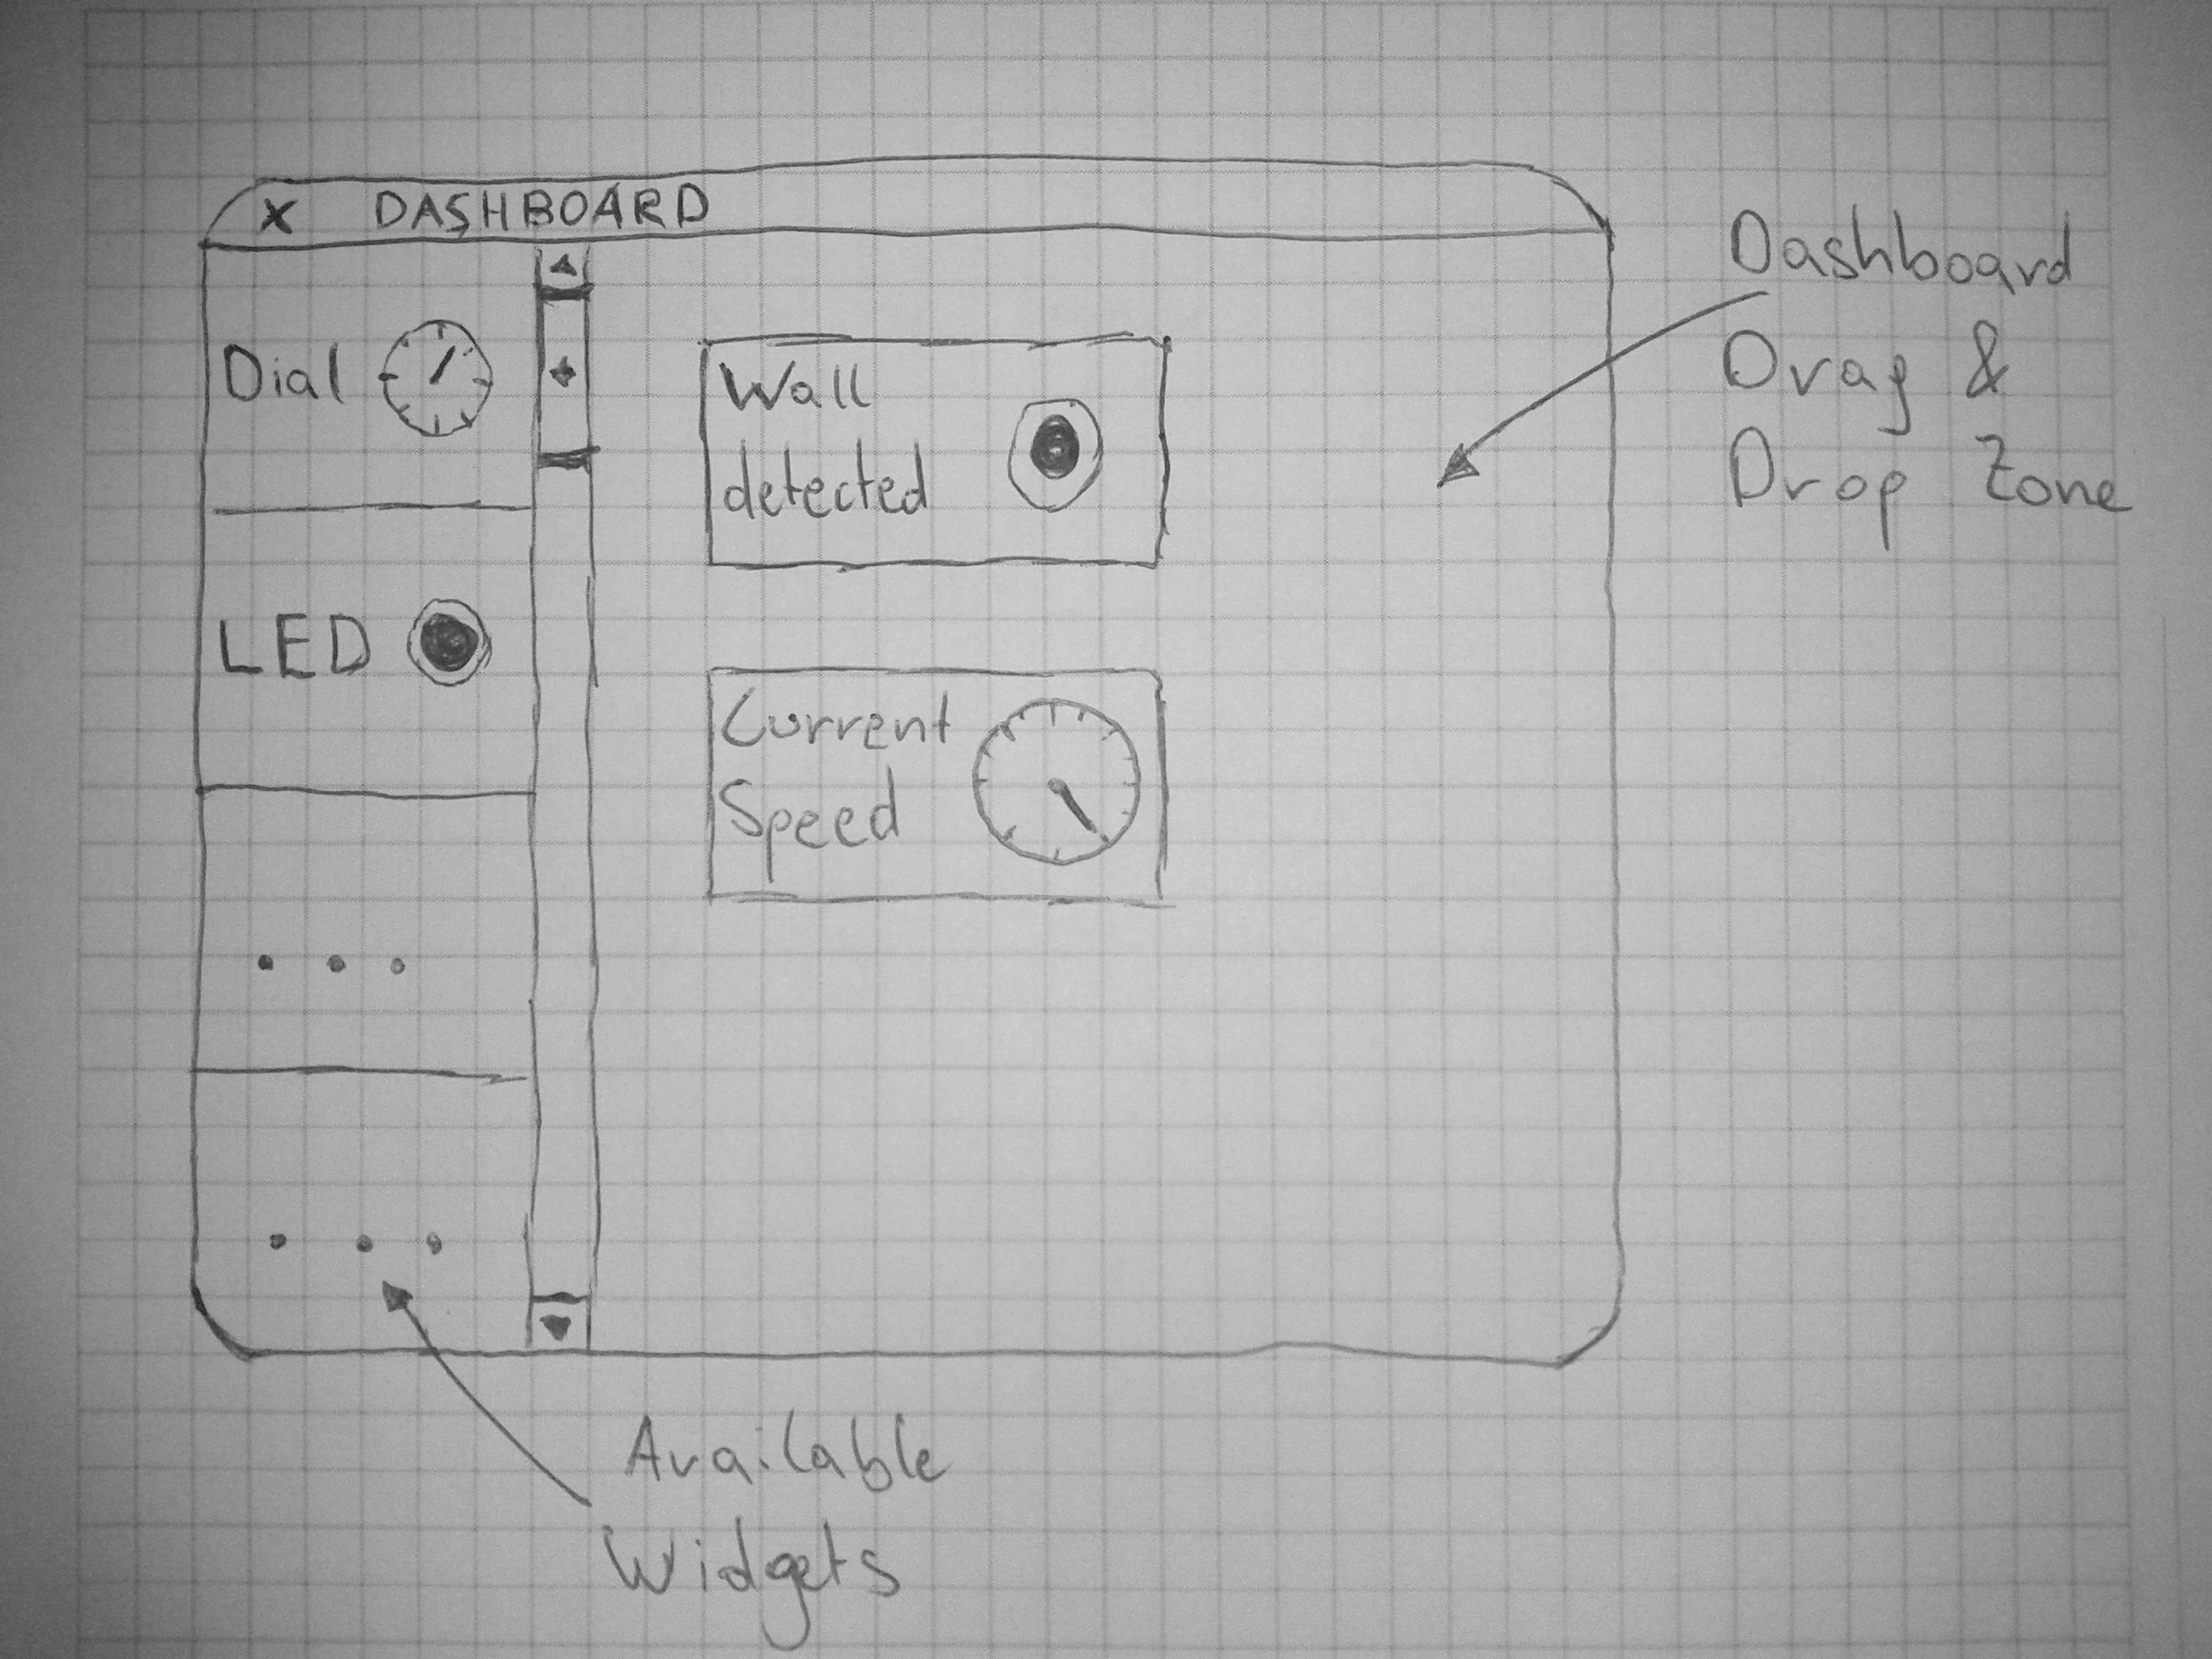
\includegraphics[width=\textwidth]{img/initial_gui_mockup.jpg}
  \caption{Paper mockup for the graphical interface.}
  \label{gui_mockup}
\end{figure}

Each item in the list on the left (Figure~\ref{gui_mockup}) represents one type of visualization, this can be as simple as a dial for numeric values or more complex visualizations for more concrete data like a map visualization. Although the design of the user interface does not restrict the types of visualizations, it is intended for simple and abstract data, since other tools like RViz (see Section~\ref{rviz}) are more specialized for complex and spatial data required in other use cases.

\begin{figure}[htbp]
  \centering
  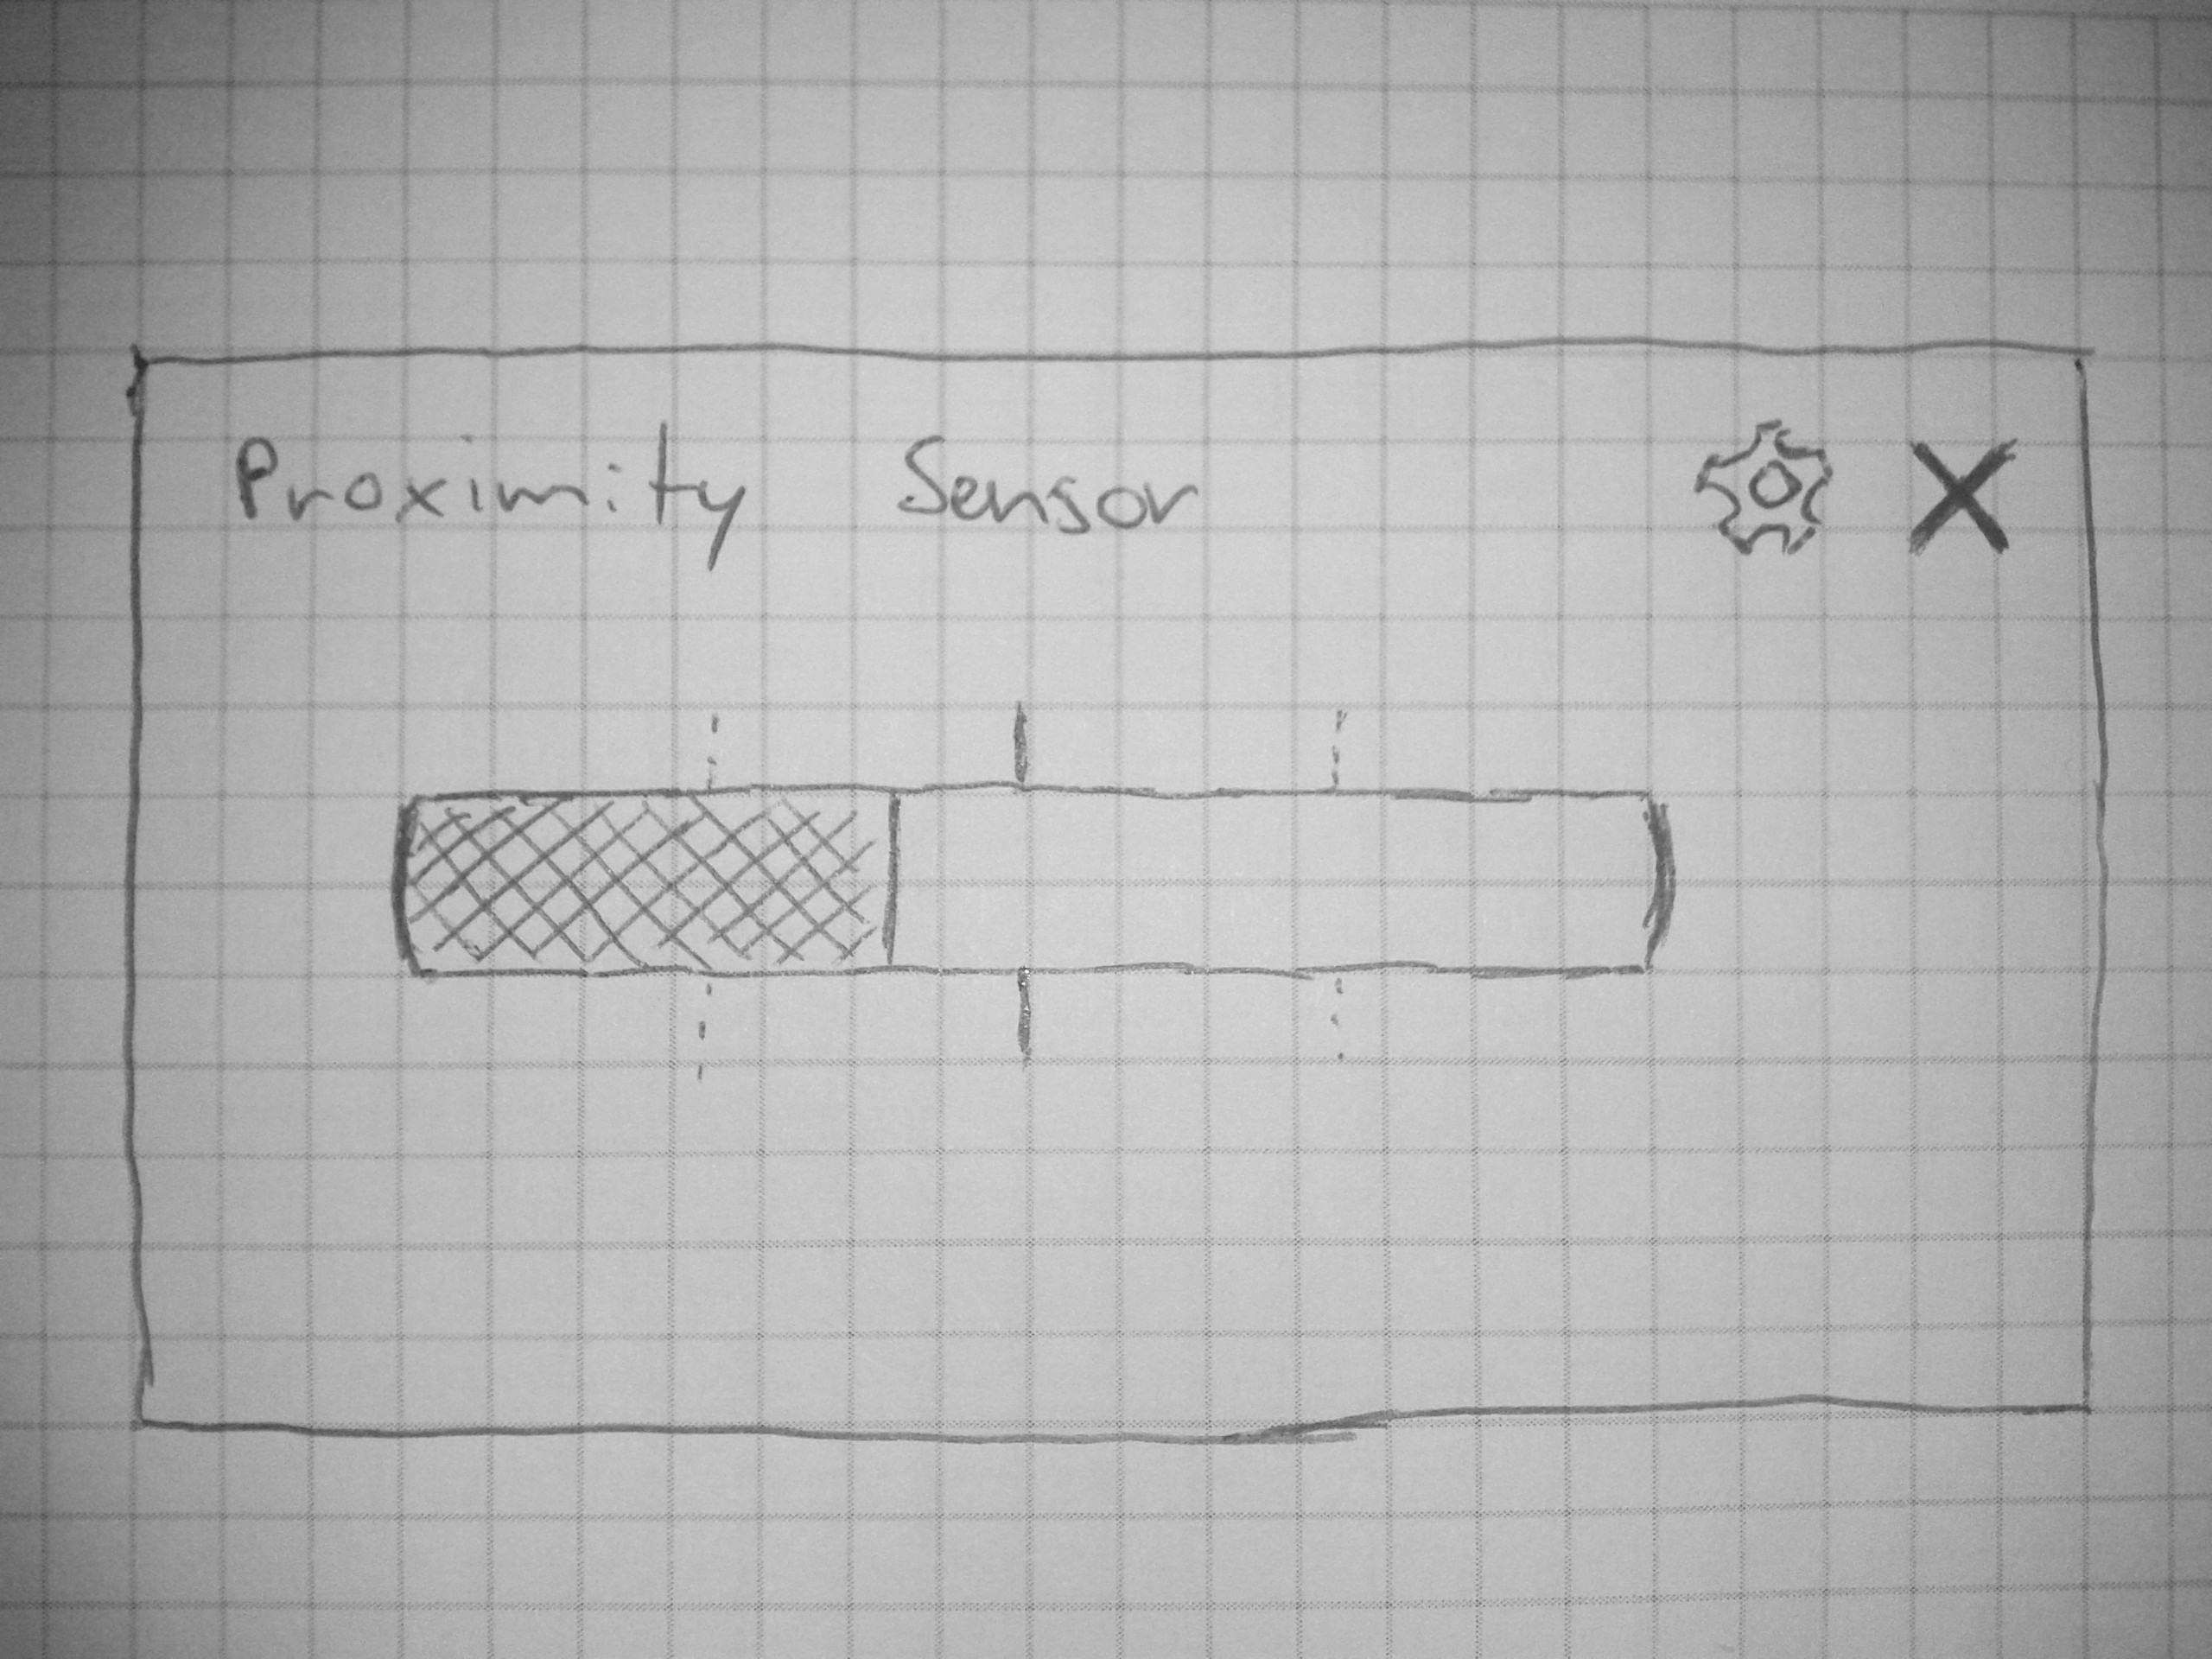
\includegraphics[width=.5\textwidth]{img/initial_widget_mockup.jpg}
  \caption{Paper mockup for a visualization widget.}
  \label{widget_mockup}
\end{figure}

Figure~\ref{widget_mockup} shows an early mockup of a visualization widget on the dashboard. This exemplary visualization widget has the form of a progress bar where numeric values can be visualized. Dials, meters, thresholds, compasses and LEDs could be other simple visualizations widgets. A more complex example for a visualization widget is the laser scan visualization as shown in Figure~\ref{laser_viz}.
%The widgets can be hooked up to data providers and will be updated once a new value is available.

\begin{figure}%[thpb]
  \centering
  \framebox{
    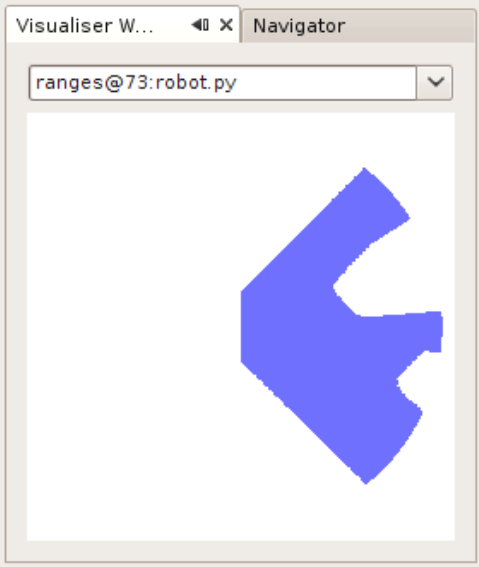
\includegraphics[width=0.4\textwidth]{img/laser_visualization.png}
  }  
  \caption[A possible laser visualization.]{A possible laser visualization, as shown in Luke Gumbley's paper on realtime debugging (Fig.~7). \cite{Gumbley2009}}
  \label{laser_viz}
\end{figure}

\subsection{Architecture}
The currently available robotic frameworks mostly rely on a communication middleware that abstracts from the concrete communication channels. This communication infrastructure can be used by the proposed debugging system to access data without the need to develop a dedicated communication layer for debugging.

The user interface mockup shown in Figure~\ref{gui_mockup} already indicates the modular design of visualizations that can be added to the dashboard canvas. The modular approach makes it easy to extend the system with more visualizations in the future and it gives developers the choice how data is visualized. Each visualization widget contains a different form of visualization. This visualization widget handles the graphical part of the visualization, stores information about the data connection and other settings and encapsulates the communication with the middleware. The connection with the communication middleware is established through an adapter which notifies the widget if the data has changed or new data is available. This makes it easy to exchange the communication adapter if the communication protocol changes or the implementation targets a different robotic framework which has a different communication structure. This reduces the coupling between the visualizations and the data collection. Although the dashboard needs to know which widgets are currently on the dashboard, the widgets itself are independent of the dashboard. The decentralized approach allows easier integration of a plugin infrastructure since the dashboard itself does not need to be modified to show additional visualization widgets.

%Figure~\ref{communication_diagram} shows how the modular visualization widgets connect to the communication middleware through the adapter. The robot modules at the bottom of the diagram publish data of some kind: either data which is needed to communicate with other modules or data specifically emitted for debugging. The visualizations can connect to both kinds of data through the middleware.

\begin{figure}%[htbp]
  \centering
  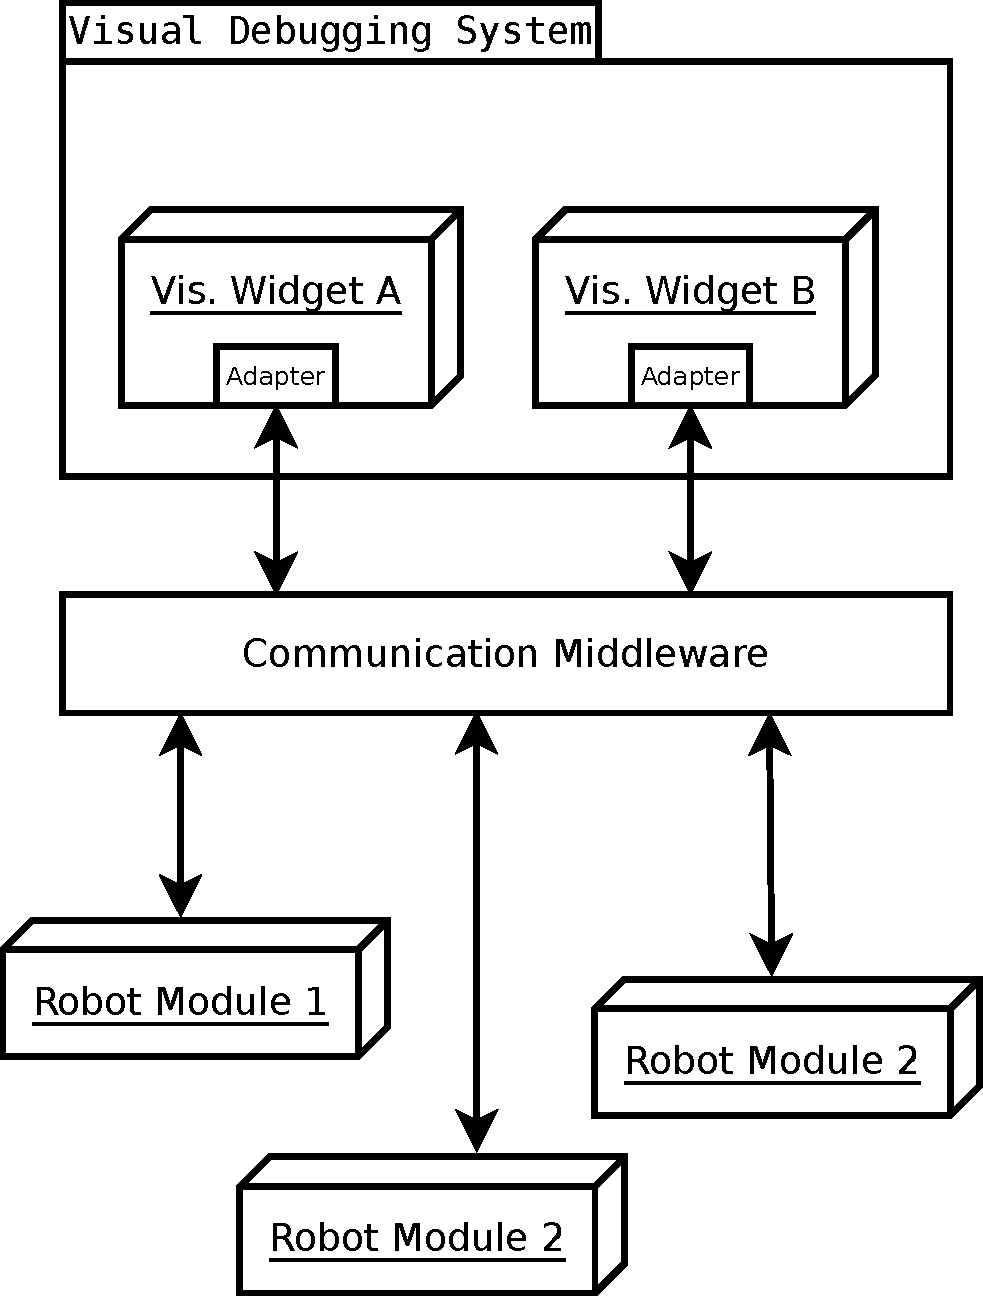
\includegraphics[width=.5\textwidth]{diagrams/communication_diagram}
  \caption{Communication diagram}
  \label{communication_diagram}
\end{figure}

Since the visualization widgets can connect directly to the communication middleware, existing data used for inter-module-communication can be visualized as well as dedicated debugging data. What kind of data is visualized is irrelevant for the visual debugging system and allows to also use it as pure monitoring tool to keep track of existing communication data between modules. Figure~\ref{communication_diagram} shows how different robot modules communicate with each other through the communication middleware. The adapter instances in the visualization widgets can connect to the communication using the same principle used for inter-module-communication. It is transparent to the visualization widgets whether the visualized data comes from eavesdropping on communication between modules or is dedicated debugging data. 

ROS has been examined as an example for a robotic framework with a communication middleware, since some of the ROS tools were already presented in Chapter~\ref{debugging_in_robotics}. The publish/subscribe style communication in ROS successfully decouples the sender from the receiver of messages \cite{Eugster2003}. Since this principle also appears in other frameworks it should be simple to implement an adapter that connects to the communication middleware of a specific robotic framework. If the communication structure is fundamentally different in the target robotic framework, some more work might be required to decouple the visualization from the data collection.

\subsection{Object Model}
\label{object_model_section}

\begin{figure}%[thpb]
  \centering
  \framebox{
    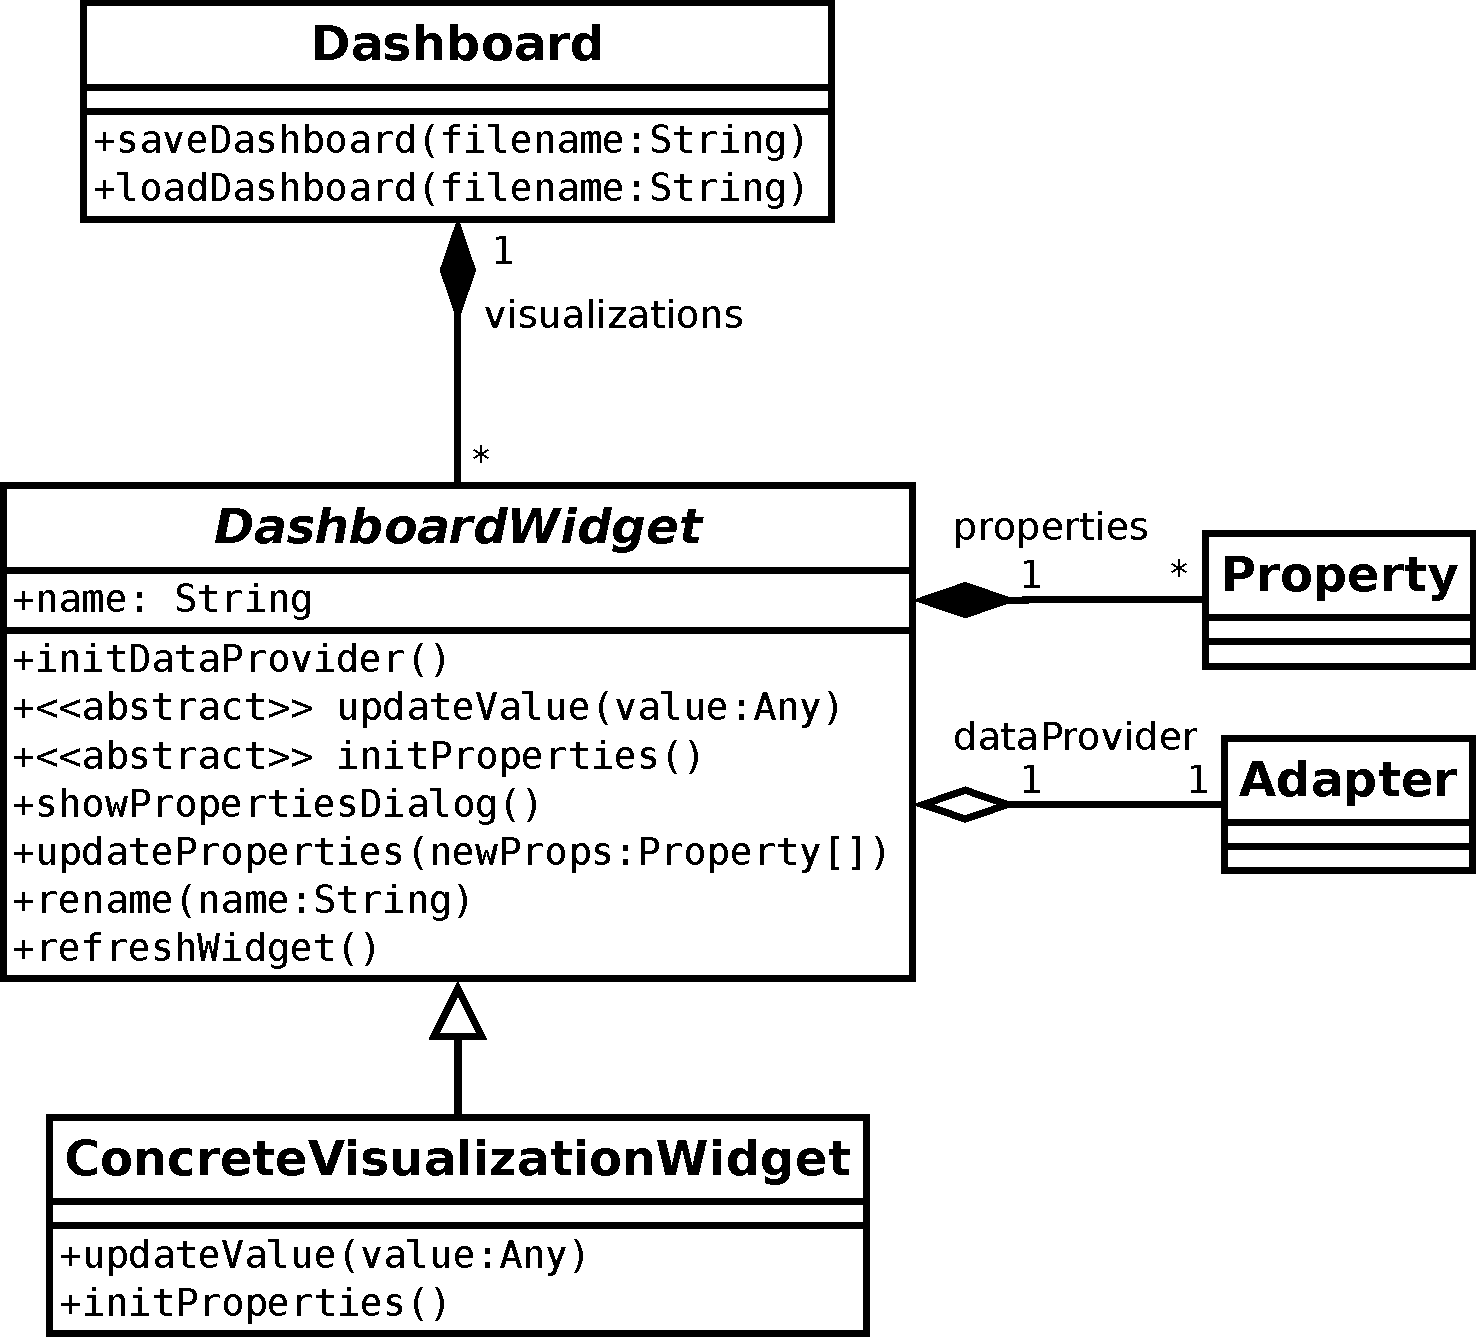
\includegraphics[width=0.9\textwidth]{diagrams/class_overview.pdf}
  }  
  \caption{Extendible object model.}
  \label{class overview}
\end{figure}

The object model shown in Figure~\ref{class overview} was designed to make it easy to extend the debugging system with more visualization widgets. The abstract \textbf{DashboardWidget} class implements the general methods that are the same for every widget. Its internal method structure allows subclasses to overwrite only some parts of functionality, without the need to rewrite most of the other methods. This allows easy integration of a plugin framework at a later stage, where third party widget developers only need to implement the specific parts of the new widget they want to provide and the common parts are handled by the default implementation in \textbf{DashboardWidget}. The class \textbf{ConcreteVisualizationWidget} stands for a possible visualization widget that implements the abstract methods from \textbf{DashboardWidget}. Each visualization widget has to subclass \textbf{DashboardWidget} to make use of \textbf{DashboardWidget}s default implementation framework.

The data provider setup and the properties management are also implemented in the \textbf{DashboardWidget} class, because they will likely be the the same for most widgets. The main reason is to hide the technical details from a third party plugin developer to make his life easier. The plugin developer only needs to specify which properties his widget has in \verb+initProperties()+, the default implementation of \verb+updateProperties()+ saves the new properties and notifies the widget to update the user interface through \verb+updateWidget()+. The \textbf{DashboardWidget} automatically supports numeric, text and float properties. If more specific properties are needed the plugin developer can overwrite the properties-specific methods in \textbf{DashboardWidget} to provide an implementation tailored to this specific widget.

The \textbf{Adapter} class in Figure~\ref{class overview} can be seen as a black box that takes care of the communication with the communication middleware from the respective robotic framework. The \textbf{Adapter} connects to the communication middleware and waits for new data. If new data is published it notifies the visualization widget to update the value of the widget through \verb+updateValue(value: Any)+. The diagram in Figure~\ref{update_value_sequence} shows how the \verb+updateValue+ method gets passed to the \textbf{Adapter} upon initialization to decouple the user interface from the application logic. When the \textbf{Adapter} receives a new value through the publish/subscribe communication middleware, it passes the value on to the \textbf{DashboardWidget} which updates the user interface.

\begin{figure}%[thpb]
  \centering
  \framebox{
    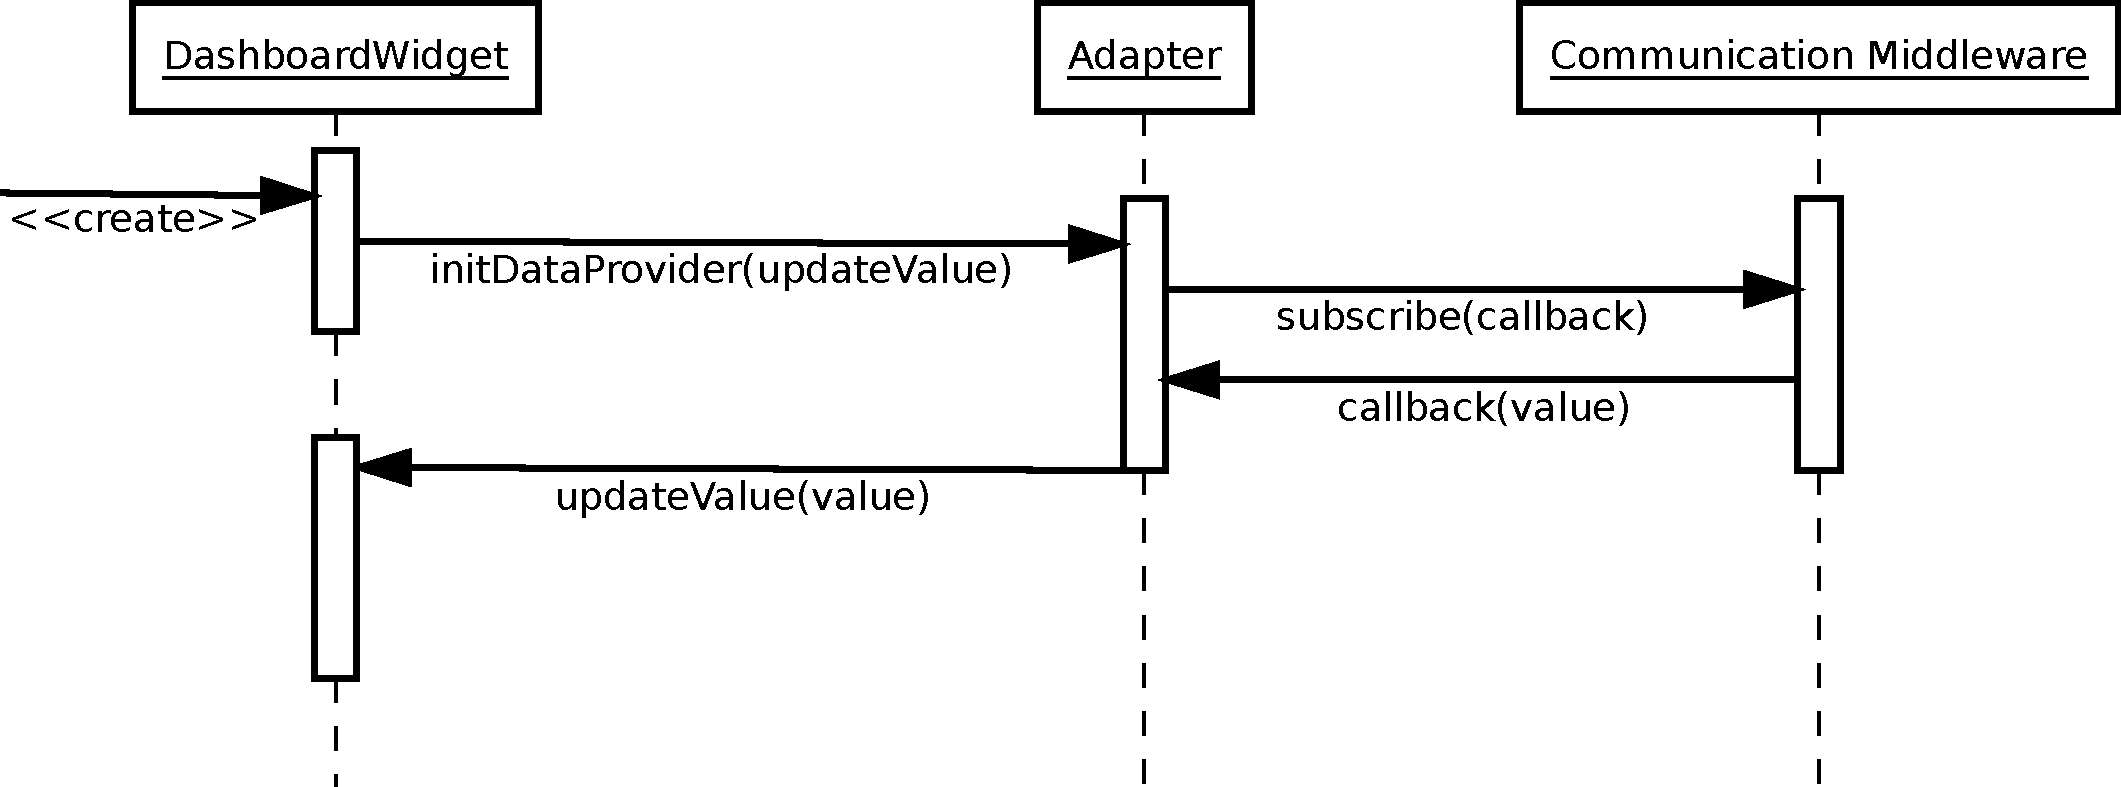
\includegraphics[width=.95\textwidth]{diagrams/update_value_sequence.pdf}
  }  
  \caption{Decoupling the user interface from the application logic with callbacks.}
  \label{update_value_sequence}
\end{figure}


\subsection{Plugin Architecture}
\label{plugin_architecture_section}
The architecture and object model presented in the previous sections aim to make it easy to extend the visual debugging system with further widgets. To allow third party developers to add their visualizations a plugin architecture will be presented in this section. The plugin architecture allows to add new visualization widgets in form of plugins, without the need to modify the source code directly.

The diagram in Figure~\ref{plugin_architecture_diagram} shows the object design of the plugin architecture. Plugins can be loaded and unloaded through the \textbf{PluginManager} class. The \textbf{PluginManager} class keeps a list of all plugins and populates the toolbox where plugins can be selected from (see Figure~\ref{gui_mockup}). The plugin itself contains the implementation of a visualization widget which is subclassed from \textbf{DashboardWidget} and some additional meta information about the plugin.

\begin{figure}[htb]
  \centering
  \framebox{
    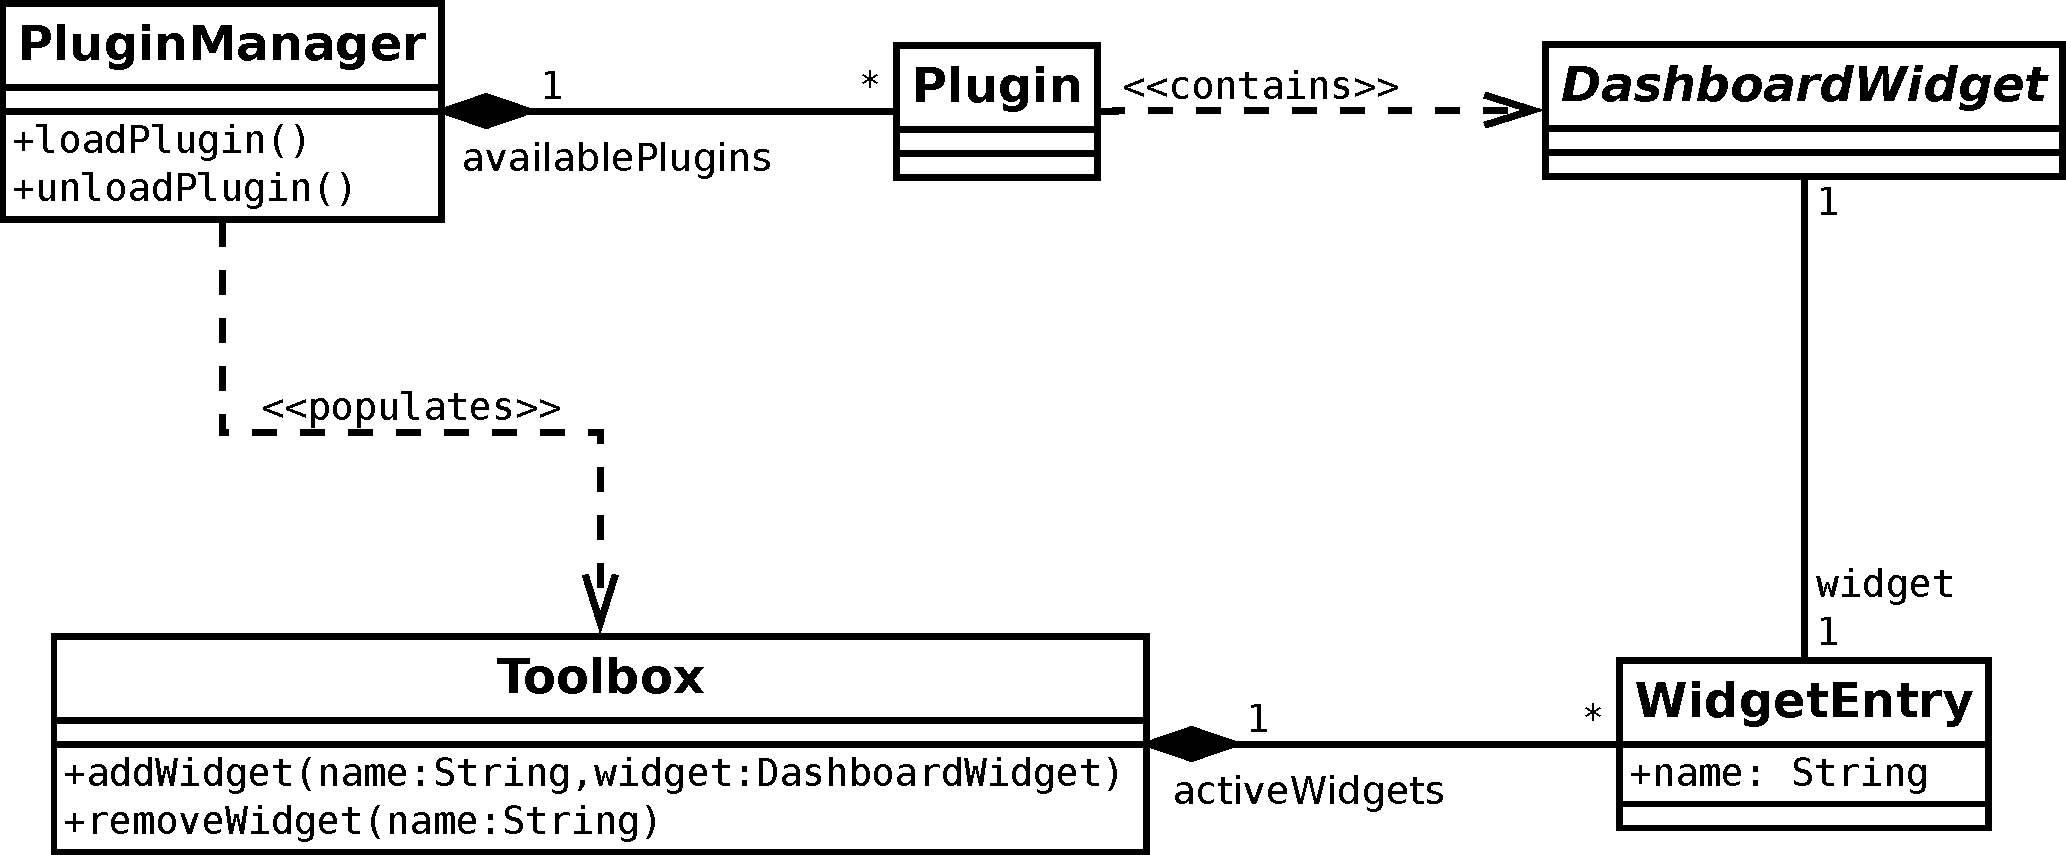
\includegraphics[width=0.9\textwidth]{diagrams/plugin_architecture.pdf}
  }  
  \caption{Plugin architecture overview.}
  \label{plugin_architecture_diagram}
\end{figure}
